\documentclass[]{article}
\usepackage{amsmath}
\usepackage{amsfonts}
\usepackage{amssymb}
\usepackage[utf8]{inputenc}
\usepackage{graphicx}
\usepackage{geometry}
\usepackage{color}
\usepackage{siunitx} %\SI{44.9}{\celsius}
\usepackage[german]{babel}
\usepackage{fancyref}
\usepackage{circuitikz} %für Stromkreise
\long\def \/*#1*/{} %Kommentare mit \/* ---- */
\geometry{
	a4paper,
	left=25mm,
	right=25mm,
	top=25mm,
	bottom=25mm,
}
\pagenumbering{arabic}

\title{Messung der Schallgeschwindigkeit in Luft}
\date{02.01.18}
\author{Mate Farkas, Patrick Schillings}
\begin{document}
	
	
	\tableofcontents
	
	\noindent\makebox[\linewidth]{\rule{\textwidth}{0.4pt}}
	
	\section{Versuchsziele}
	
	Das Ziel des Versuchs ist es, die Schallgeschwindigkeit in Luft zu messen. Dazu sollen drei verschiedene Methoden verwendet werden, einmal die Auftragung einer Laufstrecke innerhalb einer Laufzeit, einmal die Messung von Resonanzfrequenzen innerhalb eines Rohres bekannter Länge und einmal durch die Messung der Wellenlänge bei bekannter Frequenz einer stehenden Welle.
	
	\section{Grundlagen} %TODO: Als eigenes?
	
	Die Wellenlänge $\lambda$ und die Frequenz $f$ beschreiben eine Schallwelle mit der Geschwindigkeit
	
	\begin{equation}
		v_{Schall}=\lambda*f=\frac{\Delta s}{\Delta t}.
		\label{e1}
	\end{equation}
	
	Für stehende Wellen auf der Länge $L$ mit zwei festen Enden gilt
	
	\begin{equation}
		L=n*\frac{\lambda}{2}
		\label{e2}
	\end{equation}
	oder umgeformt
	\begin{equation}
	v_{Schall}=\frac{2L}{n}*f
	\label{e3} 
	\end{equation}	
	mit der Ordnung n.
	
	%Bild stehende Welle
	
	\section{Versuche}
	
	\subsection{Kalibration des Wegaufnehmers}
	\subsubsection{Aufbau und Durchführung}
	
	Um die stehende Welle im Rohr in den späteren Teilen zu untersuchen, wurde der Wegaufnehmer gegenüber eines Messbandes Klasse II kalibriert. Ziel dieses Teilversuches ist damit, einen funktionalen Zusammenhang zwischen den am Wegaufnehmer (der wie ein Schiebewiderstand charakterisieren lässt) gemessenen Widerstand und die Längenverschiebung L. Dazu wurde der {\color{red} {Schiebekopf}} auf die 0.5 cm - Marke des Messbandes gelegt und der Widerstand mithilfe eines Teststroms gemessen. Dies wurde in 5-cm Schritten wiederholt, wovon die Rohdaten sich in der folgenden Tabelle zusammenfassen lassen:
	
	\begin{center}
		
		\begin{tabular}{|c|c|c|c|c|c|c|}
			\hline 
			Abstand s in cm & 0.5 & 5.5 & 10.5 & 15.5 & 20.5 & 25.5 \\ 
			\hline 
			Widerstand R in $\Omega$ & 1.685 & 1.375, & 1.06 & 0.755, & 0.44 & 0.125 \\ 
			\hline 
		\end{tabular} 
	\end{center}
	
	\subsubsection{Auswertung}
	
	Die Messpunkte Widerstand R gegen Position L des Mikrophons kann man in Abb.\ref{Kalib_Reg} erkennen. Mit diesen wurde eine lineare Regression $L=k*R+L_0$ durchgeführt, die ebenfalls dargestellt ist. Als Fehler gehen hierbei die Ablese- beziehungsweise Digitalisierungslimitierungen ein: $L_{err}=0.1cm/2$ und $R_{err}=0.005k\Omega/\sqrt{12}$ ein. Der konstante systematische Fehler des Maßbandes spielt keine Rolle, da später nur die Steigung des Graphen, sowie Längendifferenzen wichtig werden.      
     
    Das Ergebnis der Regression beträgt $(16.040\pm0.042)cm/k\Omega*R+(2.957\pm0.044)cm$ mit einem $X^2/f \approx 2.704/4 \approx 0.676$. Der Residuenplot dazu ist in Abb.\ref{Kalib_Res} dargestellt. Man erkennt, dass alle Fehler $\sqrt{k^2*R_{err}^2+L_{err}^2}$ etwa im Rahmen einer Standardabweichung um die Funktion gestreut sind.\\   
                   
   	\begin{figure}
    	\begin{center}
    		\includegraphics[scale=0.9]{Images/Kalibrierung_Regression.pdf}
    		\caption{Regressionsgerade der Kalibrierung}             
    		\label{Kalib_Reg}               
    	\end{center}            
    \end{figure} 
    
	\begin{figure}
	\begin{center}
		\includegraphics[scale=0.9]{Images/Kalibrierung_Residuum.pdf}
		\caption{Residuenplot der Kalibrationsgeraden}
		\label{Kalib_Res}
	\end{center}
	\end{figure}
	\subsection{Messung von Laufzeit und Laufstrecke eines Signals}
	Ein Piezo-Hochtöner wird auf einer Geraden mit einem darauf verschiebbaren Mikrophon fest angebracht. Für verschiedene Mikrophonpositionen wird die Zeitdifferenz zwischen Tonerzeugung und Tonempfang gemessen. Die Postionen des Mikrophons werden über einen Wegaufnehmer bestimmt.
	
	In der ersten Versuchsreihe wurden die Laufzeiten und -wege wie in Abb.\ref{Va_Reg} aufgenommen. Hier hilft der zweite Teil von Formel \ref{e1}, um die Geschwindigkeit des Schalls in Luft mit einer linearen Regression $s(t)=v_{Schall}*t+s_0$ zu bestimmen. 
	
	\begin{figure}
	\begin{center}
		\includegraphics[scale=0.9]{Images/VA_Regression.pdf}
		\caption{Regression zur Ermittlung der Schallgeschwindigkeit}
		\label{Va_Reg}
	\end{center}
	\end{figure}	
	Das Residuum kann man in Abb.\ref{Va_Res} sehen. Die Werte liegen gestreut um die Gerade, so wie es auch sein sollte, allerdings 
	\begin{figure}
	\begin{center}
		\includegraphics[scale=0.9]{Images/VA_Residuum.pdf}
		\caption{Residuum der Geradenanpassung}
		\label{Va_Res}
	\end{center}
	\end{figure}	


	
	\subsection{Messung von Resonanzfrequenzen einer stehenden Welle}
	\subsubsection{Aufbau und Durchführung}
	\subsubsection{Auswertung}
	
	\subsection{Messung der Wellenlänge einer stehenden Welle}
	\subsubsection{Aufbau und Durchführung}
	\subsubsection{Auswertung}
	
	Die Messergebnisse kann man in Abb.\ref{Vc_Roh} betrachten.

	\begin{figure}
	\begin{center}
		\includegraphics[scale=0.9]{Images/VC_Roh.png}
		\caption{Schallamplitude bei bestimmten Positionen}
		\label{Vc_Roh}
	\end{center}
	\end{figure}
	

	\section{Ergebnisse}
	\subsection{Temperaturauswertung}
		Die theoretische Schallgeschwindigkeit in Luft kann in Abhängigkeit von der Temperatur (in K) hergeleitet werden:
	\begin{equation}
	v_{theo}=\sqrt{\frac{R*\kappa}{M_{Mol}}*T}
	\label{v(T)}
	\end{equation}
	, wobei die allgemeine Gaskonstante $R=8.3145 \frac{J}{mol*K}$, der Adiabatenexponent für Luft $\kappa=\frac{7}{5}$ und deren molare Masse $M_{Mol}=28.984*10^{-3} \frac{kg}{mol}$ bereits ziemlich genau bekannt sind.
	Nun soll die Temperatur in Abhängigkeit von der Zeit bestimmt werden.\\
	Zu Beginn der Versuchsreihe um 17:05 Uhr wurde die Temperatur gemessen, ebenso wie zwischen den Experimenten und am Ende. Ungefähre Zeiten (die Endzeiten), wann die Experimente genau stattfanden, finden sich in Abb.\ref{Temp_Zeiten}. Da keine eigentliche Messung (ohne Vorbereitung) länger als 15 Minuten dauerte, wird der statistische Fehler auf die Zeit zu $\sigma_t=15min$ abgeschätzt. Der Digitalisierungsfehler der Temperatur ist $\sigma_T=\SI{0.1}{\celsius}/\sqrt{12}$.\\
	17:05 Uhr wird als Zeitnullpunkt festgesetzt. Es wird in Minuten gezählt. Die Daten der drei Messungen sind in Abb.\ref{Temp_vorn} bis Abb.\ref{Temp_hinten} zu finden. Darin wurde bereits der Mittelwert eingezeichnet. Die Histogramme der Temperaturverteilungen zu den verschiedenen Zeiten sind von Abb.\ref{Temp_vorn_hist}
 	bis Abb.\ref{Temp_hinten_hist} dargestellt. Man kann sehen, dass sie gaußverteilt sind und deren Mittelwerte, Standardabweichungen und systematischen Fehler berechnen. So findet man schließlich drei Messpaare mitsamt Fehler:
 	
 	\begin{center}
 	\begin{tabular}{c|c|c}
 		$t/min$ & $T/\SI{}{\celsius}$ & $\sigma_T/\SI{}{\celsius}$\\
 		\hline
 		0 & 22.7811 & 0.0031\\
 		\hline 
 		86 & 23.7975 & 0.0029\\
 		\hline
 		160 & 23.9467 & 0.0029\\
 	\end{tabular}
 	\end{center}
 	
 	Ausprobiert wurden nun sowohl eine lineare Regression als auch die Anpassung einer Exponentialfunktion durch vorheriges logarrithmieren, wobei letzteres etwas besser funktionierte. Es ergibt sich der Zusammenhang
 	\begin{equation}
 	T(t)=e^{c*t+b} *\SI{1}{\celsius}
 	\label{T(t)}
 	\end{equation}
	mit $c=(31.6\pm8.1)*10^{-5}\SI{}{\frac{1}{\minute}}$ und $b=3.1312\pm0.0085$ (vgl. Abb.\ref{Temp_Fit}).
	In Abb.\ref{Temp_Res} findet sich noch das Residuum dazu, das allerdings bei drei Messpaaren nur soweit aussagekräftig ist, alsdass die Punkte ungefähr eine Standardabweichung von der Regression entfernt liegen. Das bestätigt auch der $X^2$-Wert, der mit $X^2\approx2.26$ bei einem Freiheitsgrad nicht unwahrscheinlich ist (vgl. entsprechende Tabellen).
	
	%Fehlerfortpflanzung
	
	
	\begin{figure}
	\begin{center}
		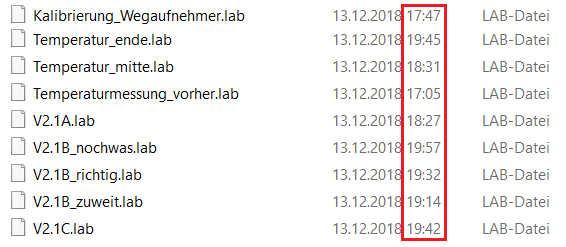
\includegraphics[scale=0.9]{Images/Messreihenendzeiten.png}
		\caption{Zeiten, zu denen die Experimente stattfanden}
		\label{Temp_Zeiten}
	\end{center}
	\end{figure}
	%\section{Anhang} ?
	
	
	\begin{figure}
	\begin{center}
		\includegraphics[scale=0.9]{Images/Rauschmessung_vor_den_Messungen.pdf}
		\caption{Rauschmessung der Temperatur vor den Messungen}
		\label{Temp_vorn}
	\end{center}
	\end{figure}	

	\begin{figure}
	\begin{center}
		\includegraphics[scale=0.9]{Images/Rauschmessung_in_der_Mitte.pdf}
		\caption{Rauschmessung der Temperatur zwischen Experimenten}
		\label{Temp_mitte}
	\end{center}
	\end{figure}

	\begin{figure}
	\begin{center}
		\includegraphics[scale=0.9]{Images/Rauschmessung_nach_den_Messungen.pdf}
		\caption{Rauschmessung der Temperatur nach den Messungen}
		\label{Temp_hinten}
	\end{center}
	\end{figure}

	\begin{figure}
	\begin{center}
		\includegraphics[scale=0.9]{Images/Temperatur_vor_den_Messungen.pdf}
		\caption{Histogramm der Temperatur vor den Messungen}
		\label{Temp_vorn_hist}
	\end{center}
	\end{figure}

	\begin{figure}
	\begin{center}
		\includegraphics[scale=0.9]{Images/Temperatur_in_der_Mitte.pdf}
		\caption{Histogramm der Temperatur zwischen den Messungen}
		\label{Temp_mitte_hist}
	\end{center}
	\end{figure}

	\begin{figure}
	\begin{center}
		\includegraphics[scale=0.9]{Images/Temperatur_nach_den_Messungen.pdf}
		\caption{Histogramm der Temperatur nach den Messungen}
		\label{Temp_hinten_hist}
	\end{center}
	\end{figure}

	\begin{figure}
	\begin{center}
		\includegraphics[scale=0.9]{Images/Temperatur_Verlauf.pdf}
		\caption{Anpassung einer Exponentialfunktion an den Temperaturverlauf}
		\label{Temp_Fit}
	\end{center}
	\end{figure}

	\begin{figure}
	\begin{center}
		\includegraphics[scale=0.9]{Images/Temperatur_Residuum.pdf}
		\caption{Residuenplot der linearen Regression an die logarrithmierte Temperatur}
		\label{Temp_Res}
	\end{center}
	\end{figure}




	
\end{document}
